\documentclass[11pt,fleqn]{article}
\linespread{1.3}
\usepackage{parskip}
\setlength{\parindent}{0pt} %no paragraph indentation
\setlength{\parskip}{2.1ex plus 0.2ex minus 0.2ex} %3x paragraph spacing
\usepackage{geometry}
\geometry{a4paper,left=30mm,right=25mm,top=20mm,bottom=20mm} %margin spacing
\usepackage{fancyhdr}
\pagestyle{fancy}
\fancyhf{}
\renewcommand{\headrulewidth}{0pt}
\rfoot{\thepage}

\usepackage[pdftex]{graphicx} %so that eps files may be included
\usepackage{amsmath}
\usepackage{amssymb}
\usepackage{amsthm}
\usepackage{float}

% Theorems, definitions etc.
\newtheoremstyle{defstyle}
  {10pt} % Space above
  {0pt} % Space below
  {} % Body font
  {} % Indent amount
  {\bfseries} % Theorem head font
  {.} % Punctuation after theorem head
  {0.5em} % Space after theorem head
  {} % Theorem head spec (can be left empty, meaning `normal')
\theoremstyle{defstyle}
\newtheorem{defn}{Definition}[section]
\newtheorem{rmrk}{Remark}[section]

\begin{document}
%Title page
\begin{titlepage}

\center % Center everything on the page
 
%----------------------------------------------------------------------------------------
%	HEADING SECTIONS
%----------------------------------------------------------------------------------------

\textsc{\LARGE University of Pretoria}\\[1.5cm] % Name of your university/college
\textsc{\Large Department of Mathematics and Applied Mathematics}\\[0.5cm] % Major heading such as course name
\textsc{\large WTW 795: Essay}\\[3.5cm] % Minor heading such as course title

%----------------------------------------------------------------------------------------
%	TITLE SECTION
%----------------------------------------------------------------------------------------


\huge \textsc{Finite Element Approximation for Convection, Diffusion and Reaction systems in a Tubular Reactor} \\[3.5cm]
 
%----------------------------------------------------------------------------------------
%	AUTHOR SECTION
%----------------------------------------------------------------------------------------

\begin{minipage}{0.4\textwidth}
\begin{flushleft} \large
\emph{Author:}\\
St. Elmo Wilken % Your name
\end{flushleft}
\end{minipage}
~
\begin{minipage}{0.4\textwidth}
\begin{flushright} \large
\emph{Student Number:} \\
29034133 
\end{flushright}
\end{minipage}\\[2cm]

\begin{minipage}{0.4\textwidth}
\begin{center} \large
\emph{Supervisor:} \\
Prof. van Rensburg % Supervisor's Name
\end{center}
\end{minipage} \\[2cm]

%----------------------------------------------------------------------------------------
%	DATE SECTION
%----------------------------------------------------------------------------------------

{\large \today}\\[3cm] % Date, change the \today to a set date if you want to be precise

\vfill % Fill the rest of the page with whitespace

\end{titlepage}

%Abstract and Keywords
\begin{center}
\Large Finite Element Approximation for Convection, Diffusion and Reaction Systems in a Tubular Reactor \\[0.5cm]
\large St. Elmo Wilken \\
29034133
\end{center}

\begin{abstract}
Insert abstract...
\end{abstract}

\textsc{\small KEYWORDS:} \small Finite Element Method, diffusion, convection, reaction, tubular reactor
\tableofcontents
\pagenumbering{gobble}

\newpage
\pagenumbering{arabic}
\section{Introduction}

\section{Model Derivation}
In this section the general convection, diffusion and reaction (CDR) continuum equation is developed. Furthermore, the accompanying energy balance necessitated by the reaction component of the resultant model is also derived. For the purposes of this project a tubular reactor geometry is assumed; thus the model is derived with respect to the (more natural) cylindrical coordinate system. 

\begin{defn}
Diffusion is the spontaneous mixing of molecules by random thermal motion. It gives rise to motion of a chemical species relative to the motion of the mixture.
\end{defn}

In the absence of other gradients, molecules of a single species will always diffuse from regions of higher concentration to regions of lower concentration. This concentration gradient results in a molar flux of the species.

\begin{defn}
For species A the molar flux is denoted by $\mathbf{W}_A$ and has units of $\frac{moles}{time \times area}$. The molar flux is a vector quantity and can be expressed as $\mathbf{W}_A = W_A|_r \mathbf{e}_r + W_A|_\theta \mathbf{e}_\theta + W_A|_z \mathbf{e}_z$ in cylindrical coordinates. The molar flow rate is related to the molar flux and cross-sectional area by $F_A|_i = A_c|_i \times W_A|_i$ where $i$ indicates the component of interest. 
\end{defn}

The basis of the model's derivation rests on the conservation of mass principle. A consequence of this assumption is the mole balance: barring a reaction, the number of moles of a species is conserved within a given control volume. The mole balance for the reacting species A is derived with reference to the control volume depicted in Figure \ref{fig_vol_element}.

\begin{figure}[H] 
\centering
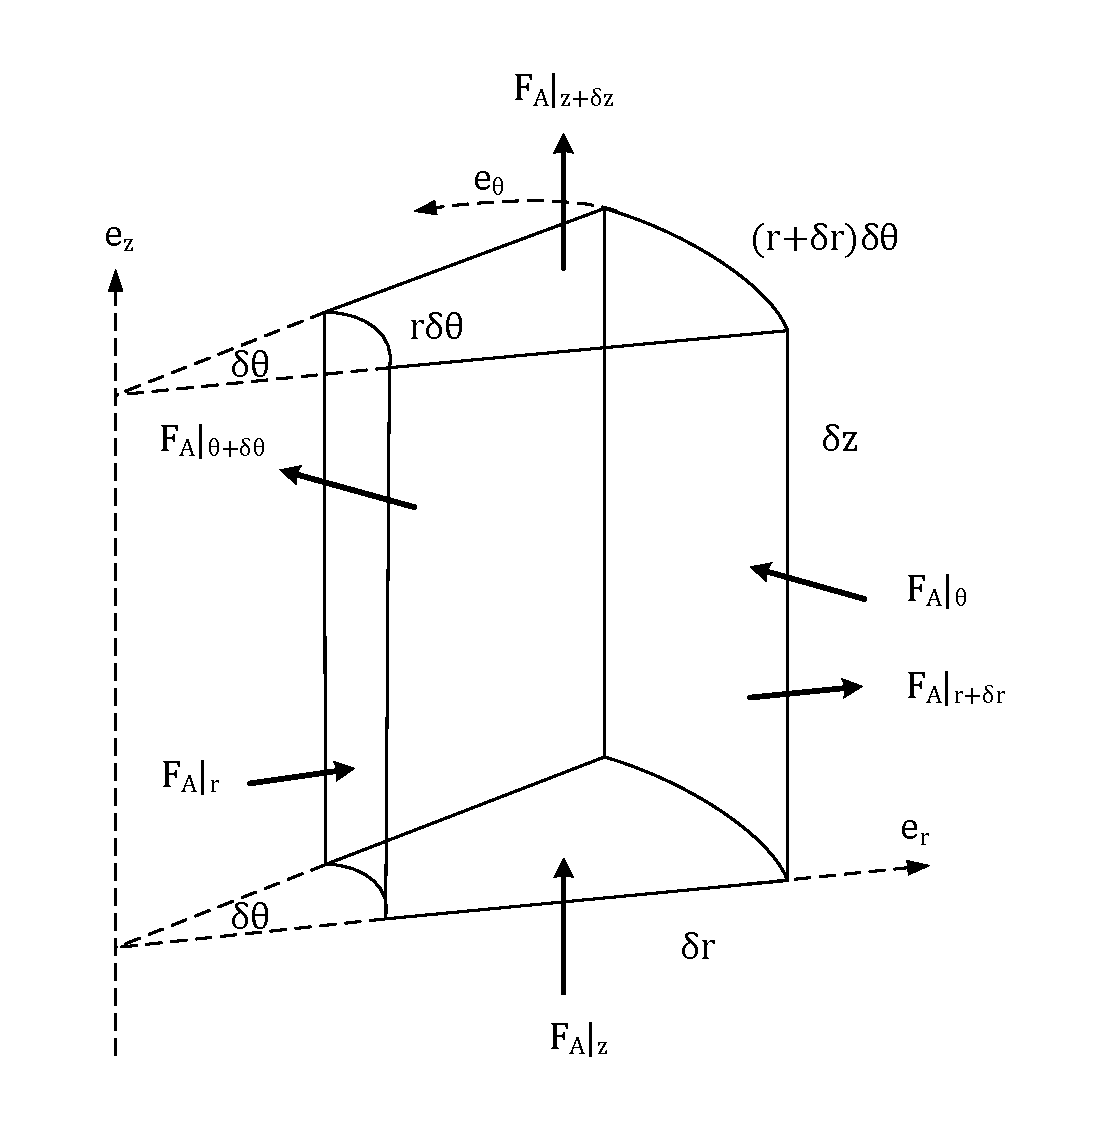
\includegraphics[scale=0.5]{./pics/volume_element}
\caption{Control volume for a tubular reactor} 
\label{fig_vol_element}
\end{figure}

The mole balance is shown in (\ref{eq_mole_balance}) where $r_A$ indicates the generation or consumption of species A due to reaction and $C_A$ is the concentration of species A in the mixture. The term on the right hand side of (\ref{eq_mole_balance}) represents the accumulation of species A in the control volume ($\delta V$).
\begin{equation}
\sum_{i=r, \theta, z}[F_A|_i(i) - F_A|_i(i+\delta i)] + r_A \delta V = \delta V \frac{\partial C_A}{\partial t}
\label{eq_mole_balance}
\end{equation}
Consider the molar flow rate in the $\mathbf{e}_r$ direction. By using the definition of molar flux and the linear approximation of $F_A|_r(r+\delta r)$ we have (\ref{eq_far}).
\begin{equation}
\begin{aligned}
F_A|_r(r) &= W_A|_r(r) r \delta \theta \delta z \\
F_A|_r(r+\delta r) &= (W_ A|_r(r) + \frac{\partial W_A|_r(r)}{\partial r} \delta r)(r+\delta r)\delta \theta \delta z + h(\delta r)
\end{aligned}
\label{eq_far}
\end{equation}
For the linear approximation we have $\lim_{\delta r \to 0} ||\delta r||^{-1}||h(\delta r)|| = 0 $ and consequently for sufficiently small $\delta r$ we have (\ref{eq_far2}).  
\begin{equation}
F_A|_r(r) - F_A|_r(r+\delta r)  = - (W_ A|_r(r)  + \frac{\partial W_A|_r(r)}{\partial r}r) \delta r \delta \theta \delta z
\label{eq_far2}
\end{equation}
In a similar manner, consider the molar flow rate in the $\mathbf{e}_\theta$ direction. By again using the definition of molar flux and the linear approximation of $F_A|_\theta(\theta+\delta \theta)$ we have (\ref{eq_fat}).
\begin{equation}
\begin{aligned}
F_A|_\theta(\theta) &= W_A|_\theta(\theta) \delta r \delta z \\
F_A|_\theta(\theta + \delta \theta) &= W_A|_\theta(\theta) \delta r \delta z + \frac{\partial W_A|_\theta(\theta)}{r \partial \theta}\delta \theta\delta r \delta z + h(\delta \theta)
\end{aligned}
\label{eq_fat}
\end{equation}
Again, for sufficiently small $\delta \theta$ we have (\ref{eq_fat2}).
\begin{equation}
F_A|_\theta(\theta) - F_A|_\theta(\theta + \delta \theta) =- \frac{\partial W_A|_\theta(\theta)}{r \partial \theta}\delta \theta\delta r \delta z
\label{eq_fat2} 
\end{equation}
Finally, consider the molar flow rate in the $\mathbf{e}_z$ direction. By using the definition of molar flux, the linear approximation of $F_A|_z(z+\delta z)$ and approximating the cross-sectional area normal to $\mathbf{e}_z$ in Figure \ref{fig_vol_element} as a trapezium we have (\ref{eq_faz}).
\begin{equation}
\begin{aligned}
F_A|_z(z) &= W_A|_z(z) r \delta r \delta \theta \\
F_A|_z(z + \delta z) &= W_A|_z(z) r \delta r \delta \theta + \frac{\partial W_A|_z(z)}{\partial z}r \delta z \delta r \delta \theta + h(\delta z)
\end{aligned}
\label{eq_faz}
\end{equation}
Finally, for sufficiently small $\delta z$ we have (\ref{eq_faz2}).
\begin{equation}
F_A|_z(z) - F_A|_z(z + \delta z) = - \frac{\partial W_A|_z(z)}{\partial z}r \delta z \delta r \delta \theta
\label{eq_faz2}
\end{equation}
Substituting (\ref{eq_far2}), (\ref{eq_fat2}) and (\ref{eq_faz2}) into (\ref{eq_mole_balance}) results in (\ref{eq_mb2}). Note that for sufficiently small $\delta r$ we have $\delta V \approx r \delta \theta \delta r \delta z$.
\begin{equation}
- (W_ A|_r(r)  + \frac{\partial W_A|_r(r)}{\partial r}r) \delta r \delta \theta \delta z - \frac{\partial W_A|_\theta(\theta)}{r \partial \theta}\delta \theta\delta r \delta z - \frac{\partial W_A|_z(z)}{\partial z}r \delta z \delta r \delta \theta + r_A \delta V = \delta V \frac{\partial C_A}{\partial t}
\label{eq_mb2}
\end{equation}
Dividing through by $r \delta \theta \delta r \delta z$ results in (\ref{eq_mb3}) which is equivalent to (\ref{eq_mb4}).
\begin{equation}
-\frac{1}{r} W_A|_r - \frac{\partial W_A|_r}{\partial r} - \frac{1}{r^2}\frac{\partial W_A|_\theta}{\partial \theta} - \frac{\partial W_A|_z}{\partial z}+ r_A  = \frac{\partial C_A}{\partial t}
\label{eq_mb3}
\end{equation}
\begin{equation}
-\frac{1}{r} \frac{\partial (rW_A|_r)}{\partial r} - \frac{1}{r^2}\frac{\partial W_A|_\theta}{\partial \theta} - \frac{\partial W_A|_z}{\partial z}+ r_A  = \frac{\partial C_A}{\partial t}
\label{eq_mb4}
\end{equation}
It is now necessary to make modelling assumptions. Firstly, we will neglect any variations in the rotational direction (modelled by assuming $\frac{\partial W_A|_\theta}{\partial \theta} \approx 0$).

Secondly, we assume that Fick's Law is valid, that the diffusivity ($D_{AB}$) is constant and that the total concentration of the system is constant. This last assumption limits us to considering only reactions which conserve the total number of moles e.g. $A \rightarrow B$ or $A + B \rightarrow 2C$ etc..

Thirdly, we assume that the convection in the radial direction is negligible and that the velocity profile of molar flow in the axial direction only varies in the radial direction ($U(z,r)=U(r)$). These assumptions are not particularly strong but nevertheless simplify the model considerably. The resultant constitutive equations are shown in (\ref{eq_fick}).  
\begin{equation}
\begin{aligned}
W_A|_z &= -D_{AB}\frac{\partial C_A}{\partial z} + C_A U(r) \\
W_A|_r &= -D_{AB}\frac{\partial C_A}{\partial r}  
\end{aligned}
\label{eq_fick}
\end{equation} 
Substituting (\ref{eq_fick}) into (\ref{eq_mb3}) results in the model (\ref{eq_cdr}) we will use for this project \cite{fogler}.
\begin{equation}
D_{AB}(\frac{1}{r}\frac{\partial}{\partial r}(r\frac{\partial C_A}{\partial r}) + \frac{\partial^2 C_A}{\partial z^2}) - U_z\frac{\partial C_A}{\partial z} + r_A = \frac{\partial C_A}{\partial t}
\label{eq_cdr}
\end{equation}
Up to now not much has been said about the reaction term $r_A$. Typically $r_A$ is formulated as a rate equation based on experimental evidence modelling reaction kinetics. It is possible for the rate ``law" to be quite complex in character. A class of commonly encountered expressions for forward, irreversible reactions are based on power law kinetics \cite{levenspiel}. Power law kinetics usually take the form $-r_A=k(T)[C_A]^M$ for reactions of the form $A \rightarrow B$ or $-r_A=k(T)[C_A]^M[C_B]^N$ for reactions of the form $A + B \rightarrow 2C$ with $M,N$ usually a non-negative integer less than 3. The factor $k(T)$ is called the rate constant even though it is not a constant (it depends quite strongly on temperature). The Arrhenius equation is a very commonly used empirical function which describes the temperature dependence of the rate constant. It is typically expressed by (\ref{eq_arrhenius}) where $E$ is the activation energy, $R$ the ideal gas constant and $k_a$ is the pre-exponential factor at the reference temperature $T_a$. 
\begin{equation}
k(T) = k_a e^{(\frac{E}{R}(\frac{1}{T_a} - \frac{1}{T}))}
\label{eq_arrhenius}
\end{equation} 
It is prudent (in practice a necessity) to attempt to model the temperature profile of the reactor. We start the derivation by considering the first law of thermodynamics for an open system again applied to the control volume in Figure \ref{fig_vol_element}. In (\ref{eq_ftd}) $F_{i0}$ and $F_{i}$ denotes the molar flow of species $i$ into and out of the control volume respectively, and similarly with the energy $E$. The law states that the rate of change of energy in a system is the sum of the heat flow ($\dot{Q}$) to the system minus the work done ($\dot{W}$) by the system plus the rate of energy transferred due to flow (the last two terms). 
\begin{equation}
\frac{d E_{syst}}{dt} = \dot{Q} - \dot{W} + \sum F_{i0}E_{i0} -\sum F_{i}E_{i}
\label{eq_ftd}
\end{equation}
\begin{rmrk}
More precisely the flow terms should be vector valued due to the choice of the control volume. This is suppressed at the moment for the sake of clarity. Additionally, unless otherwise stated, $\sum$ is actually the sum over all species in the control volume i.e. $\sum_{i=1}^{N}$ where $i=1$ would indicate species 1 etc.. 
\end{rmrk}
It is customary to separate the work term into shaft and flow work terms as in (\ref{eq_work}). In this equation $\hat{V}_i$ indicates the specific molar volume of species $i$.
\begin{equation}
\dot{W} = -\sum F_{i0}P\hat{V}_{i0} + \sum F_{i}P\hat{V}_{i} + \dot{W}_s
\label{eq_work} 
\end{equation}
Substituting this into (\ref{eq_ftd}) we have (\ref{eq_ftd2}).
\begin{equation}
\frac{d E_{syst}}{dt} = \dot{Q} - \dot{W}_s + \sum F_{i0}(E_{i0}+P\hat{V}_{i0}) -\sum F_{i}(E_{i}+P\hat{V}_{i})
\label{eq_ftd2}
\end{equation}
Now by assuming that the energy $E_i$ is approximately equal to the internal energy $U_i$ (this assumption implies that the potential energy, kinetic energy etc. of the system is dwarfed by the internal energy), and by making use of the definition of enthalpy, $H_i = U_i + P\hat{V}_i$, we can simplify (\ref{eq_ftd2}) to (\ref{eq_ftd3}).
\begin{equation}
\frac{d E_{syst}}{dt} = \dot{Q} - \dot{W}_s + \sum F_{i0}H_{i0} -\sum F_{i}H_{i}
\label{eq_ftd3}
\end{equation} 
Now consider the left hand side of \ref{eq_ftd3}. By definition $E_{syst} = \sum N_iE_i$ where $N_i$ is the number of moles of species $i$ in the system. By using the definition of concentration ($C_i = \frac{N_i}{\delta V}$) and noting that due to our earlier assumptions $E_i = H_i - P\hat{V}_i$  we have (\ref{eq_syse}).
\begin{equation}
\frac{d E_{syst}}{dt} = \delta V \frac{\partial}{\partial t}(\sum C_i (H_i - P\hat{V}_i))
\label{eq_syse}
\end{equation}
Expanding the right hand side of (\ref{eq_syse}), assuming constant pressure and making use of the definitions of the specific molar volume ($\sum \hat{V}_iC_i = 1$) and enthalpy at constant pressure ($dH_i = C_{p_i}dT$) we have (\ref{eq_syse2}).
\begin{equation}
\frac{d E_{syst}}{dt} = \delta V \sum C_i C_{p_i} \frac{\partial T}{\partial t} + \delta V \sum H_i \frac{\partial C_i}{\partial t} 
\label{eq_syse2}
\end{equation}
If we neglect shaft work we have the general form of the first law of thermodynamics we will be using in (\ref{eq_gfl}).  
\begin{equation}
\frac{\dot{Q}}{\delta V} + \frac{1}{\delta V}(\sum F_{i0}H_{i0} -\sum F_{i}H_{i}) =\sum C_i C_{p_i} \frac{\partial T}{\partial t} + \sum H_i \frac{\partial C_i}{\partial t}
\label{eq_gfl}
\end{equation}
It now becomes necessary to consider the components of volume element  in Figure \ref{fig_vol_element} to take the derivation further.
\begin{rmrk}
Since we neglected rotational variance in the final form of the CDR equation we will immediately neglect the angular component of the volume element in the following analysis.  
\end{rmrk}
Consider energy flow terms $\frac{1}{\delta V}(\sum F_{i0}H_{i0} -\sum F_{i}H_{i})$ from (\ref{eq_gfl}) in the $\mathbf{e}_r$ and $\mathbf{e}_z$ directions for a particular species A. Using the same analysis as with the CDR derivation we have (\ref{eq_tcp1}).
\begin{equation}
\begin{aligned}
F_{A0}|_r H_{A0}(r) - F_{A}|_rH_{A}(r+\delta r) &= -(W_A|_r H_A(r) + \frac{\partial W_A|_r H_A(r)}{\partial r}r)\delta r \delta \theta \delta z \\
F_{A0}|_z H_{A0}(z) - F_{A}|_z H_{A}(z+\delta z) &= -\frac{\partial W_A|_z H_A(z)}{\partial z}r \delta r \delta \theta \delta z   
\end{aligned}
\label{eq_tcp1}
\end{equation}
Summing over all the components in the control volume and noticing that this (\ref{eq_tcp1}) resembles the flux terms in (\ref{eq_mb3}) we can rewrite (\ref{eq_gfl}) into (\ref{eq_tcp2}).
\begin{equation}
\frac{\dot{Q}}{\delta V} - \frac{1}{r}\frac{\partial}{\partial r}(r\sum W_i|_r H_i) - \frac{\partial}{\partial z}(\sum W_i|_z H_i) =\sum C_i C_{p_i} \frac{\partial T}{\partial t} + \sum H_i \frac{\partial C_i}{\partial t}
\label{eq_tcp2}
\end{equation}
Assuming that we can neglect the change in enthalpy in the radial direction and expanding the derivatives we have (\ref{eq_tcp3}).
\begin{equation}
\frac{\dot{Q}}{\delta V} - \sum H_i (\frac{1}{r}\frac{\partial}{\partial r}(r W_i|_r)+\frac{\partial}{\partial z}(W_i|_z)) - \sum W_i|_z \frac{\partial H_i}{\partial z} =\sum C_i C_{p_i} \frac{\partial T}{\partial t} + \sum H_i \frac{\partial C_i}{\partial t}
\label{eq_tcp3}
\end{equation}
Now note that we can substitute in (\ref{eq_mb4}) (without the rotational term) to get to (\ref{eq_tcp4}).
\begin{equation}
\frac{\dot{Q}}{\delta V} - \sum H_i r_i - \sum W_i|_z \frac{\partial H_i}{\partial z} =\sum C_i C_{p_i} \frac{\partial T}{\partial t}
\label{eq_tcp4}
\end{equation}
Now assume that $\sum H_i r_i = -H_{rxn}r_A$ where $H_{rxn}$ is the heat of reaction.
\begin{rmrk}
A more thorough derivation will show that it is not necessary to assume that $\sum H_i r_i = -H_{rxn}r_A$ since it follows from the definition of the reaction rate. However, we assume it for the sake of brevity. We also assume that the heat of reaction is constant in this project. Physically it is the heat added by the reaction to the system per mole reacted where the limiting species is A.
\end{rmrk}
We also assume that $W_i|_z \approx U_z C_i$ which is equivalent to assuming that the convective component of the axial flux dominates the diffusional component. With these assumptions we have (\ref{eq_tcp5}).
\begin{equation}
\frac{\dot{Q}}{\delta V} + H_{rxn}r_A - U_z\sum C_{p_i}C_i \frac{\partial T}{\partial z} =\sum C_i C_{p_i} \frac{\partial T}{\partial t}
\label{eq_tcp5}
\end{equation}
Firstly, consider the case where the heat added to the system does not depend on the spatial dimensions (if $\dot{Q}$ is non-zero it is called non-adiabatic). In this case we can assume that in the limit as $\delta V \rightarrow 0 $ we have that $\frac{\dot{Q}}{\delta V} = U_ha(T_a-T)$ where $U_h$ is the heat transfer coefficient and $a = \frac{\pi D}{A_c}$ with $D, A_c$ the diameter and cross sectional area of the reactor.
\begin{rmrk}
The assumption that $\frac{\dot{Q}}{\delta V} = U_ha(T_a-T)$ actually comes from a theoretical analysis of heat conduction, but since the focus of this project is on the CDR equation we just assume it. 
\end{rmrk} 
This assumption results in the one dimensional non-adiabatic energy balance for a tubular reactor shown in (\ref{eq_baltb1}).
\begin{equation}
U_ha(T_a-T) - U_z\sum C_{p_i}C_i \frac{\partial T}{\partial z} + H_{rxn}r_A = \sum C_i C_{p_i} \frac{\partial T}{\partial t}
\label{eq_baltb1}
\end{equation}
If we assume adiabatic conditions (\ref{eq_baltb1}) simplifies to (\ref{eq_baltb2}) where $X$ is the conversion of the limiting species and $C_{p_m}$ is the average heat capacity of the system (which is constant).
\begin{equation}
T = T_0 + \frac{-H_{rxn}X}{C_{p_m}}
\label{eq_baltb2}
\end{equation}
\begin{rmrk}
The adiabatic energy balance actually has its roots in a simpler energy balance but, once again, for the sake of brevity we just assume the truth of (\ref{eq_baltb2}).
\end{rmrk}
Finally, we consider the case where the heat added has both radial and axial components. By assuming that the heat term can be written in vector form $\dot{Q} = q_r A_r \mathbf{e}_r + q_z A_z \mathbf{e}_z$  where $A_r$ and $A_z$ are the cross-sectional areas, and following the same procedure as before we have (\ref{eq_heat1}).
\begin{equation}
\frac{\dot{Q}}{\delta V} = -\frac{1}{r}\frac{\partial}{\partial r}(r q_r) - \frac{\partial}{\partial z}(q_z)
\label{eq_heat1}
\end{equation}
By substituting Fourier's laws, $q_r = -k_e\frac{\partial T}{\partial r}$ and $q_z = -k_e\frac{\partial T}{\partial z}$ with $k_e$ the average coefficient of conduction of the species in the reactor, into (\ref{eq_heat1}) and combining this with (\ref{eq_tcp5}) we end up with the two dimensional non-adiabatic energy balance for a tubular reactor (\ref{eq_baltb3}).
\begin{equation}
\frac{k_e}{r}\frac{\partial}{\partial r}(\frac{r\partial T}{\partial r}) + k_e\frac{\partial ^2 T}{\partial z^2} + H_{rxn}r_A - U_z\sum C_{p_i}C_i \frac{\partial T}{\partial z} =\sum C_i C_{p_i} \frac{\partial T}{\partial t}
\label{eq_baltb3}
\end{equation}
Assuming further that the sum $\sum C_i C_{p_i} = C_{p_m}$ is constant and that we have laminar flow i.e. $U_z = 2U_0(1-(\frac{r}{R})^2) = U(r)$, we have a simplified model amenable to our purposes (\ref{eq_baltb4}).
\begin{equation}
k_e(\frac{1}{r}\frac{\partial}{\partial r}(r\frac{\partial T}{\partial r}) + \frac{\partial ^2 T}{\partial z^2}) - U(r) C_{p_m} \frac{\partial T}{\partial z} + H_{rxn}r_A = C_{p_m} \frac{\partial T}{\partial t}
\label{eq_baltb4}
\end{equation}
\begin{rmrk}
It is interesting to note the striking similarity between the two modelling equations (\ref{eq_baltb4}) and (\ref{eq_cdr}).
\end{rmrk}
\begin{rmrk}
Boundary conditions are still required to completely formulate the model but this will be addressed in the next section.
\end{rmrk}
\begin{rmrk}
In the non-adiabtic case one would also want to perform an energy balance on the cooling fluid (it would affect the $T_a$ term in (\ref{eq_baltb1}) and the boundary conditions for (\ref{eq_baltb4})) but to simplify our model even more we assume that the cooling mechanism/fluid has a much larger heat capacity than the reacting system and that it comes from an infinite reservoir at temperature $T_a$. This assumption is quite strong.
\end{rmrk}

\section{Overview}
The purpose of this project is twofold. Firstly, it serves as an introduction to the use of the Finite Element Method (FEM) for solving typical reactor modelling problems found in chemical engineering. Secondly, it investigates the error made by making an (engineering) simplification to the model.
\begin{defn}
The Aris-Taylor approximation is a procedure where the radial component of the two dimensional CDR equation is lumped with the axial component resulting in a simplified one dimensional partial differential equation. This simplification replaces the diffusion coefficient ($D_{AB}$) with a lumped diffusion coefficient ($D_a$). The lumped coefficient is defined as $D_a = D_{AB} + \frac{U^2R^2}{48D_{AB}}$. This simplification is valid only for reactors with a laminar flow profile. 
\end{defn}
This project is divided into two parts. In the first part an isothermal reactor is assumed. The full two dimensional CDR model is solved and compared to the simplified (by way of Aris-Taylor) one dimensional CDR model. In the second part the use of the FEM is illustrated for solving non-linear coupled systems. The goal of the second part is to lay the foundation for future work where the same system as before is analysed non-isothermally.

Below follows a concise motivation for problems addressed and solved in this project. 
\subsection{Isothermal Overview}
In this section we model the simple first order reaction $A \rightarrow B$ using the rate expression $-r_A=kC_A$. Since we assume isothermal conditions the rate constant is constant. The CDR equation derived earlier (for laminar flow) may be used to model this situation, it is shown in (\ref{eq_iso1}) for convenience.
\begin{equation}
D_{AB}(\frac{1}{r}\frac{\partial}{\partial r}(r\frac{\partial C_A}{\partial r}) + \frac{\partial^2 C_A}{\partial z^2}) - 2U(1-(\frac{r}{R})^2)\frac{\partial C_A}{\partial z} - kC_A = \frac{\partial C_A}{\partial t}
\label{eq_iso1}
\end{equation} 
If one simplifies the model using the Aris-Taylor approximation the model becomes (\ref{eq_iso2}).
\begin{equation}
D_a \frac{\partial^2 C_A}{\partial z^2} - U \frac{\partial C_A}{\partial z} - kC_A = \frac{\partial C_A}{\partial t}
\label{eq_iso2}
\end{equation}
As explained earlier, these two models will be compared using (\ref{eq_iso1}) as a more accurate baseline.
\subsection{Non-Isothermal Overview}
\label{section_noniso}
The isothermal assumption made in the previous subsection is not a realistic assumption. However, it does simplify the model considerably because by assuming isothermal conditions the model becomes linear and uncoupled. The non-linear non-isothermal model corresponding to (\ref{eq_iso1}) is shown in (\ref{eq_noniso1}).
\begin{equation}
\begin{aligned}
&D_{AB} \frac{\partial^2 C_A}{\partial z^2} - U(r) \frac{\partial C_A}{\partial z} - k(T)C_A 
= \frac{\partial C_A}{\partial t} \\
& k_e(\frac{1}{r}\frac{\partial}{\partial r}(r\frac{\partial T}{\partial r}) + \frac{\partial ^2 T}{\partial z^2}) - U(r) C_{p_m} \frac{\partial T}{\partial z} - H_{rxn}k(T)C_A = C_{p_m} \frac{\partial T}{\partial t} \\
&\text{with } k(T) = k_0 \exp(\frac{-E}{RT}) \text{ and } U(r)=2U(1-(\frac{r}{R})^2)
\end{aligned}
\label{eq_noniso1}
\end{equation} 
Similarly, the non-linear non-isothermal simplified model corresponding to (\ref{eq_iso2}) is shown in (\ref{eq_noniso2}).
\begin{equation}
\begin{aligned}
&D_a \frac{\partial^2 C_A}{\partial z^2} - U \frac{\partial C_A}{\partial z} - k(T)C_A 
= \frac{\partial C_A}{\partial t} \\
& k_e\frac{\partial^2 T}{\partial z^2}- U C_{p_m} \frac{\partial T}{\partial z} + H_{rxn}k(T)C_A  + U_ha(T_a-T) = C_{p_m} 
\frac{\partial T}{\partial t} \\
&\text{with } k(T) = k_0 \exp(\frac{-E}{RT})
\end{aligned}
\label{eq_noniso2}
\end{equation} 
It is clear that solving the non-linear coupled system is quite daunting. For this reason the factors which make it difficult to solve will be handled separately to lay the foundation for future work where they can be solved simultaneously. Inspection of (\ref{eq_noniso1}) or (\ref{eq_noniso2}) reveal that they each have the same difficult aspects: the non-linearity introduced by the non-isothermal assumption and the coupled system which needs to be solved simultaneously.

With this in mind consider the uncoupled non-linear problem shown in (\ref{eq_nl1}). This corresponds to an adiabatic reactor where $A \rightarrow B$. While this may seem like a major simplification it models a situation commonly encountered in practice (e.g. an insulated reactor). This problem will illustrate one way of handeling non-linear systems using the FEM.
\begin{equation}
\begin{aligned}
&D_a \frac{\partial^2 C_A}{\partial z^2} - U \frac{\partial C_A}{\partial z} - k(C_A)
C_A = \frac{\partial C_A}{\partial t} \\
& \text{with }k(C_A) = k_0 \exp(\frac{-E}{RT}) \\
& \text{and } T = T_0 + \frac{-H_{rxn} (1-\frac{C_A}{C_{A0}})}{C_{p_A}}
\end{aligned}
\label{eq_nl1}
\end{equation}  

Finally, consider the coupled problem shown in (\ref{eq_nl2}). This corresponds to an isothermal coupled reaction where $A + B \rightarrow 2C$. This problem is weakly\footnote{I use the term weakly here to indicate that it is much easier to handle than the non-linearity introduced by the Arrhenius equation in the previous problem} non-linear due to the rate equation $-r_A = kC_AC_B$.
\begin{equation}
\begin{aligned}
&D_a \frac{\partial^2 C_A}{\partial z^2} - U \frac{\partial C_A}{\partial z} - kC_AC_B 
= \frac{\partial C_A}{\partial t} \\
&D_a \frac{\partial^2 C_B}{\partial z^2} - U \frac{\partial C_B}{\partial z} - kC_AC_B 
= \frac{\partial C_B}{\partial t} \\
\end{aligned}
\label{eq_nl2}
\end{equation}

These two problems combined capture the difficulties one would encounter attempting to solve (\ref{eq_noniso1}) or (\ref{eq_noniso2}).

\section{Basis Functions}
To solve problems with the FEM it is desirable to construct basis functions with simple analytical properties. Ideally these basis functions should lend themselves to simple computational implementation for numerical integration. We consider two basis functions in this project. 

\subsection{Piecewise Linear Basis Functions}
\label{section_plb}
The so-called hat (or roof) basis functions are defined on the interval $[0,1]$ for this project. Consider a discretisation of $[0,1]$ into $n$ equidistant elements $[x_{k-1}, x_k]$ where $x_k$ indicates node $k$ with $k=0,1,...,n$. Clearly $x_0=0$ and $x_n=1$ furthermore, define the constant $h = x_1-x_0$. Now define a basis function $\phi$ over each element by (\ref{eq_basis1}).  
\begin{equation}
\begin{aligned}
&\text{For } k=1,2,...,n-1 \\
&\phi_k(x) = h^{-1}(x-x_{k-1}) \text{ for } x \in [x_{k-1}, x_k] \\
&\phi_k(x) = 1-h^{-1}(x-x_{k}) \text{ for } x \in (x_{k}, x_{k+1}] \\
&\phi_k(x) = 0 \text{ for } x \notin [x_{k-1}, x_{k+1}] \\
&\text{And otherwise} \\
&\phi_0(x) = 1- h^{-1}x \text{ for } x \in [0, x_1] \\
&\phi_0(x) = 0 \text{ for } x \notin [x_{k-1}, x_1] \\
&\phi_n(x) = h^{-1}(x-x_{n-1}) \text{ for } x \in [x_{n-1}, 1] \\
&\phi_n(x) = 0 \text{ for } x \notin [x_{n-1}, 1] \\
\end{aligned}
\label{eq_basis1}
\end{equation}
These basis functions are shown in Figure \ref{fig_linbasis} on the domain $[0,1]$. 
\begin{figure}[H] 
\centering
\includegraphics[scale=0.6]{./pics/hat}
\caption{Piecewise linear basis functions} 
\label{fig_linbasis}
\end{figure}
For reasons which will become clear later consider the matrix $K^1$ with elements defined by (\ref{eq_K1lin}).
\begin{equation}
\begin{aligned}
&K^1_{i,i+1}=K^1_{i+1,i}=\int^1_0 \partial_x(\phi_i)\partial_x(\phi_{i+1})dx = -h^{-1} \\
&K^1_{00} = K^1_{nn} = \int^1_0 \partial_x(\phi_n)\partial_x(\phi_{n})dx = h^{-1} \\
&K^1_{ii} = \int^1_0 \partial_x(\phi_i)\partial_x(\phi_{i})dx = 2h^{-1} \\
\end{aligned}
\label{eq_K1lin}
\end{equation}
This matrix then takes the form shown in (\ref{eq_K1matlin}).
\begin{equation}
K^1 = \begin{pmatrix}
h^{-1} & -h^{-1} & 0&0 & 0 &  0\\
-h^{-1} & 2h^{-1} & -h^{-1} & 0 & 0 &  0\\
0 & -h^{-1} & 2h^{-1} & -h^{-1} & 0 & 0  \\
\ddots & \ddots & \ddots & \ddots & \ddots & \ddots \\
0 & 0 & 0  & -h^{-1} & 2h^{-1}& -h^{-1} \\
0 & 0 & 0 & 0 & -h^{-1} & h^{-1}   
\end{pmatrix}
\label{eq_K1matlin}
\end{equation}
Similarly, consider the matrix $K^2$ with elements defined by (\ref{eq_K2lin}).
\begin{equation}
\begin{aligned}
&K^2_{i,i+1}=\int^1_0 \partial_x(\phi_i)\phi_{i}dx = \frac{1}{2}\\
&K^2_{i+1,i}=\int^1_0 \partial_x(\phi_i)\phi_{i+1}dx = -\frac{1}{2} \\
&K^2_{nn} = \int^1_0 \partial_x(\phi_n)\phi_{n}dx = \frac{1}{2} \\
&K^2_{00} = \int^1_0 \partial_x(\phi_n)\phi_{n}dx = -\frac{1}{2} \\
&K^2_{ii} = \int^1_0 \partial_x(\phi_i)\phi_{i}dx = 0 \\
\end{aligned}
\label{eq_K2lin}
\end{equation}
This matrix then takes the form shown in (\ref{eq_K2matlin}).
\begin{equation}
K^2 = \begin{pmatrix}
-\frac{1}{2} & \frac{1}{2} & 0& 0 & 0 &  0 \\
-\frac{1}{2} & 0 & \frac{1}{2} & 0 & 0 &  0\\
0 & -\frac{1}{2} & 0 & \frac{1}{2} & 0 & 0  \\
\ddots & \ddots & \ddots & \ddots & \ddots & \ddots \\
0 & 0 & 0  & -\frac{1}{2} & 0 & \frac{1}{2} \\
0 & 0 & 0 & 0 & -\frac{1}{2} & \frac{1}{2}   
\end{pmatrix}
\label{eq_K2matlin}
\end{equation}
Finally, consider the matrix $K^3$ with elements defined by (\ref{eq_K3lin}). 
\begin{equation}
\begin{aligned}
&K^3_{i,i+1}=K^3_{i+1,i}=\int^1_0 \phi_i\phi_{i+1}dx = \frac{h}{6} \\
&K^3_{00} = K^3_{nn} = \int^1_0 \phi_n\phi_{n}dx = \frac{h}{3} \\
&K^3_{ii} = \int^1_0 \phi_i\phi_{i}dx = \frac{2h}{3} \\
\end{aligned}
\label{eq_K3lin}
\end{equation}
This matrix then takes the form shown in (\ref{eq_K3matlin}).
\begin{equation}
K^3 = \begin{pmatrix}
\frac{h}{3} & \frac{h}{6} &0& 0 & 0 &  0\\
\frac{h}{6} & \frac{2h}{3} & \frac{h}{6} & 0 & 0 &  0\\
0 & \frac{h}{6} & \frac{2h}{3} & \frac{h}{6} & 0 & 0  \\
\ddots & \ddots & \ddots & \ddots & \ddots & \ddots \\
0 & 0 & 0  & \frac{h}{6}& \frac{2h}{3} & \frac{h}{6} \\
0 & 0 & 0 & 0 &\frac{h}{6} & \frac{h}{3}   
\end{pmatrix}
\begin{pmatrix}
u_0 \\ u_1 \\ \vdots \\ u_{n-1} \\ u_n
\end{pmatrix}
\label{eq_K3matlin}
\end{equation} 
 
\subsection{Piecewise Bilinear Basis Functions}
\label{section_pbbf}
In two dimensions the previous roof functions generalise to the piecewise bilinear basis functions. We discretise our domain $[0,1] \times [0,1]$ into $n$ rectangular elements of equal size ($\delta x, \delta y$). We number the nodes of our discretisation column wise as shown in Figure \ref{fig_pbilindomain}.
\begin{figure}[H] 
\centering
\includegraphics[scale=0.8]{./pics/pbilin}
\caption{Domain discretisation} 
\label{fig_pbilindomain}
\end{figure}
Now we define a basis function $\phi_i(x,y) = a+ bx +cy +dxy$ on each node $i$ of Figure \ref{fig_pbilindomain}. Each basis function $\phi_i$ takes on the value $1$ at node $i$ and a value of $0$ at any node not $i$. For details on the construction of the basis functions we refer the avid reader to \cite{vrb}. 

Each basis function $\phi$ is composed of four constitutive functions named $P_1, P_2, P_3$ and $P_4$ defined on the element adjacent to the basis function $\phi$ in question and with orientation shown in Figure \ref{fig_pbasis}. Each function $P$ takes on the value $1$ at the corner nearest $\phi$ and $0$ at the other corners. If the rectangle corresponding to a particular function $P$ is not in the domain it is neglected in the calculation involving that $\phi$. 
\begin{figure}[H] 
\centering
\includegraphics[scale=0.8]{./pics/basis_p}
\caption{Basis functions} 
\label{fig_pbasis}
\end{figure}
In \cite{vrb} the definitions of the constitutive basis functions $P$ are motivated. We merely state those definitions on a rectangle $[0,\delta x] \times [0, \delta y]$ in (\ref{eq_pbasisdef}). 
\begin{equation}
\begin{aligned}
&P_1(x,y) = 1 -x-y-xy \\
&P_2(x,y) = x-xy \\
&P_3(x,y) = xy \\
&P_4(x,y) = y-xy 
\label{eq_pbasisdef}
\end{aligned}
\end{equation}  
For reasons which will become clear later we consider the set of integrals and corresponding matrices in (\ref{eq_pddy}),(\ref{eq_pddx}),  (\ref{eq_pdnx}) and (\ref{eq_pnn}).
\begin{equation}
\begin{aligned}
&m^1_{i,j} = \int_0^{\delta x} \int_0^{\delta y} \partial_y(P_i) \partial_y(P_j) dydx \implies
M^1 = \frac{1}{12}\begin{pmatrix}
2d & 2s_2 & -d & 2s_2 \\
2s_1 & 2s & 2s_2 & -d \\
-d & 2s_2 & 2d & 2s_1 \\
2s_2 & -d & 2s_1 & 2d \\
\end{pmatrix} \\
&\text{with } d = 2\frac{\delta x}{\delta y}, s_1 = \frac{\delta x}{\delta y} \text{ and } s_2 = -2\frac{\delta x}{\delta y}
\end{aligned}
\label{eq_pddy}
\end{equation}
\begin{equation}
\begin{aligned}
&m^2_{i,j} = \int_0^{\delta x} \int_0^{\delta y} \partial_x(P_i) \partial_x(P_j) dydx \implies
M^2 = \frac{1}{12}\begin{pmatrix}
2d & 2s_2 & -d & 2s_2 \\
2s_1 & 2s & 2s_2 & -d \\
-d & 2s_2 & 2d & 2s_1 \\
2s_2 & -d & 2s_1 & 2d \\
\end{pmatrix} \\
&\text{with } d = 2\frac{\delta y}{\delta x}, s_1 = -2\frac{\delta y}{\delta x} \text{ and } s_2 = \frac{\delta y}{\delta x}
\end{aligned}
\label{eq_pddx}
\end{equation}
\begin{equation}
\begin{aligned}
m^3_{i,j} = \int_0^{\delta x} \int_0^{\delta y} P_i \partial_x P_j dxdy \implies
M^3 = \frac{\delta y}{12}\begin{pmatrix}
-2 & 2 & 1 & -1 \\
-2 & 2 & 1 & -1 \\
-1 & 1 & 2 & -2 \\
-1 & 1 & 2 & -2 \\
\end{pmatrix}
\end{aligned}
\label{eq_pdnx}
\end{equation}
\begin{equation}
\begin{aligned}
m^4_{i,j} = \int_0^{\delta x} \int_0^{\delta y} P_iP_j dxdy \implies
M^4 = \frac{\delta x \delta y}{36}\begin{pmatrix}
4 & 2 & 1 & 2 \\
2 & 4 & 2 & 1 \\
1 & 2 & 4 & 2 \\
2 & 1 & 2 & 4 \\
\end{pmatrix}
\end{aligned}
\label{eq_pnn}
\end{equation}
Now we are in a position to calculate matrices of the form $\int_0^1 \int_0^1 \partial_x\phi_i \partial_x\phi_j dxdy$, $\int_0^1 \int_0^1 \partial_y\phi_i \partial_y\phi_j dxdy$, $\int_0^1 \int_0^1 \phi_i \partial_x\phi_j dxdy$ and $\int_0^1 \int_0^1 \phi_i \phi_j dxdy$ for each $i=1,2,...,n$ and each $j=1,2,...,n$. Like the matrices of Section \ref{section_plb} they are each constructed in a similar manner.

Consider the construction of matrix $K^4$ which uses matrix $M^4$ as the basis of its elements as an example. For each $i=1,2,...,n$ and each $j=1,2,...,n$ we wish to compute $K^4_{i,j}$. To achieve this we ``stitch" together the four constitutive functions $P$ around node $i$ and likewise we ``stitch" together four more constitutive functions $P$ around node $j$. We sum together the overlapping constitutive functions and assign this value to $K^4_{i,j}$. This is perhaps easier to understand graphically as shown in Figure \ref{fig_mat_ex}.
\begin{figure}[H] 
\centering
\includegraphics[scale=0.8]{./pics/mat_ax}
\caption{Construction Example} 
\label{fig_mat_ex}
\end{figure} 
For example, $K^4_{1,1} = M^4_{4,4}$ because only $P_4$ overlaps with itself for nodes 1 and 1. Another example would be $K^4_{1,8} = M^4_{4,3}$ as $P_4$ overlaps with $P_3$. Another example would be $K^4_{9,9} = M^4_{1,1} + M^4_{2,2}+ M^4_{3,3}+M^4_{4,4}$ as every constitutive functions overlaps with itself. A final example is $K^4_{1,3} = 0$ as nodes 1 and 3 have no constitutive functions in common. 

A similar process is repeated for matrices $K^1, K^2$ and $K^3$. 

\section{Isothermal Problem}
In this section the isothermal models will be developed and solved using the FEM. Finally, the quality of the Aris-Taylor simplification will be analysed numerically.  
\subsection{Problem 1}
\label{section_isop1}
We start this section solving the simplified model from (\ref{eq_iso1}) because it is the least complex. The full problem is shown in (\ref{eq_p1}). It is assumed that $D_a, U, k, C_{a0},\text{ and } L$ are given because this is necessary to describe the physical reactor.  
\begin{equation}
\begin{aligned}
&D_a \frac{\partial^2 C_A}{\partial z^2} - U \frac{\partial C_A}{\partial z} - kC_A = 
\frac{\partial C_A}{\partial t} \\
&\text{Boundary Conditions:} \\
&\frac{\partial C_A}{\partial z}(z=L, \cdot) = 0\\
&C_A(z=0, \cdot) = C_{A0} \\
&\text{Initial Condition:} \\
& C_A(\cdot, t= 0) = e^{-10\frac{z}{L}}
\end{aligned}
\label{eq_p1}
\end{equation}
The boundary conditions indicate that the concentration is known at the entrance ($z=0$) of the reactor and that no reaction (change in concentration) takes place at the end ($z=L$) of the reactor. The initial condition models the situation where the reactor is filled with an inert fluid initially - the exponential term creates an artificially smooth profile for $C_{A}$ which quickly reaches zero in the start of the reactor. 

It is desirable to convert (\ref{eq_p1}) into dimensionless form. By creating the dimensionless variables $u=\frac{C_A}{C_{A0}}$, $x = \frac{z}{L}$ and $\tau = \frac{tU}{L}$ it is possible to write (\ref{eq_p1}) as (\ref{eq_p1d}).
\begin{equation}
\begin{aligned}
&\frac{\partial^2 u}{\partial x^2} - c_1 \frac{\partial u}{\partial x} - c_1c_2u = 
c_1\frac{\partial u}{\partial \tau} \\
&\text{with } c_1 = \frac{UL}{D_a} \text{ and } c_2 = \frac{kL}{U} \\
&\text{Boundary Conditions:} \\
&\frac{\partial u}{\partial x}(x=1, \cdot) = 0\\
&u(x=0, \cdot) = 1 \\
&\text{Initial Condition:} \\
& u(\cdot, \tau = 0) = e^{-10x}
\end{aligned}
\label{eq_p1d}
\end{equation}
Now suppose $v$ is an arbitrary function. By abusing our notation a little bit and using the product rule we have (\ref{eq_prodrule}).
\begin{equation}
\begin{aligned}
&(\partial_{xx}u)v + (\partial_xu)(\partial_xv) = \partial_x( (\partial_xu)v)\\
&\implies (\partial_{xx}u)v = -(\partial_xu)(\partial_xv) + \partial_x( (\partial_xu)v)
\end{aligned}
\label{eq_prodrule}
\end{equation}
By multiplying the modelling equation in (\ref{eq_p1d}) by $v$ and using (\ref{eq_prodrule}) we have (\ref{eq_p1d2}).
\begin{equation}
 -(\partial_xu)(\partial_xv) + \partial_x( (\partial_xu)v) - c_1(\partial_xu)v - c_1c_2uv = c_1(\partial_{\tau}u)v 
\label{eq_p1d2}
\end{equation}
Now if we integrate over the domain $[0, 1]$ and apply the Fundamental Theorem of Calculus we have (\ref{eq_p1d3}).
\begin{equation}
\int_0^1 (-(\partial_xu)(\partial_xv) - c_1(\partial_xu)v - c_1c_2uv)dx + [(\partial_xu(x, \cdot))v(x, \cdot)]^1_0 = \int^1_0 c_1(\partial_{\tau}u)v dx
\label{eq_p1d3}
\end{equation}
From the boundary conditions we have that $\partial_xu(1,\cdot)=0$ and by making $v$ less arbitrary i.e. $v \in \{v : v(0, \cdot)=0 \} = T$ equation (\ref{eq_p1d3}) simplifies to the variational form in (\ref{eq_p1d4}).
\begin{equation}
\int_0^1 (-(\partial_xu)(\partial_xv) - c_1(\partial_xu)v - c_1c_2uv)dx = \int^1_0 c_1(\partial_{\tau}u)v dx
\label{eq_p1d4}
\end{equation}
Now let $B(u, v) = \int_0^1 (-(\partial_xu)(\partial_xv) - c_1(\partial_xu)v - c_1c_2uv)dx$ and $(c_1(\partial_{\tau}u),v)_0 = \int^1_0 c_1(\partial_{\tau}u)v dx$. From the theory of partial differential equations, if we can find a unique function $u$ with $u(0, \cdot)=1$ which satisfies (\ref{eq_p1d5}) for all $v \in T$ we have the solution of (\ref{eq_p1d}).
\begin{equation}
B(u, v) = (c_1(\partial_{\tau}u),v)_0
\label{eq_p1d5}
\end{equation}
For the purposes of this project we will assume the existence and uniqueness of such a function. While it is certainly within the realm of possibilities to find an analytic solution to (\ref{eq_p1d5}) we will rather attempt to find an approximate solution using the FEM.

Recall the definition of the piecewise linear basis functions ($\phi$) defined in Section \ref{section_plb}. We assume that the function $u^h =\sum^n_{k=0} u_k(t) \phi_k(x)$ which by construction lies in the span $S^h=\text{span}(\phi_0,...,\phi_n)$ can approximate $u$. We reformulate the variational problem in (\ref{eq_p1d5}) by using the Galerkin approximation: find $u^h \in S^h$ such that for $S^h_0=\{\phi_1, \phi_2,...,\phi_n \}$ (\ref{eq_p1d6}) holds.
\begin{equation}
B(u^h, \phi) = (c_1(\partial_{\tau}u^h),\phi)_0~~\forall \phi \in S^h_0
\label{eq_p1d6}
\end{equation} 
\begin{rmrk}
Note the difference between $S^h$ and $S^h_0$. Clearly $S^h_0=S^h\setminus \{\phi_0\}$: it was required that the test functions satisfy $v(0)=0$ which $\phi_0$ does not. 
\end{rmrk}
Recall that $B(u, v) = \int_0^1 (-(\partial_xu)(\partial_xv) - c_1(\partial_xu)v - c_1c_2uv)dx$. Substituting the Galerkin approximation into this expression we have (\ref{eq_p1d7}).
\begin{equation}
B(u^h, \phi_i) = \int_0^1 (-(\partial_xu^h)(\partial_x\phi_i) - c_1(\partial_xu^h)\phi_i - c_1c_2u^h\phi_i)dx \text{ for } i=1,2,...,n
\label{eq_p1d7}
\end{equation}
Now we will consider each term of (\ref{eq_p1d7}) separately. Firstly, consider $\int_0^1 -(\partial_xu^h)(\partial_x\phi_i)dx$ for each $i=1,2,...,n$ as shown in (\ref{eq_lindd}).
\begin{equation}
\begin{aligned}
\int_0^1 -(\partial_xu^h)(\partial_x\phi_i)dx &= \int_0^1 -(\partial_x \sum_{k=0}^{n} u_k\phi_k)(\partial_x\phi_i)dx \\
&= \int_0^1 -\sum_{k=0}^{n} u_k(\partial_x\phi_k)(\partial_x\phi_i)dx \\
&= \begin{cases}
\int_{[x_{i-1},x_{i+1}]}-\sum_{k=i-1}^{i+1} u_k(\partial_x\phi_k)(\partial_x\phi_i)dx &\text{ for } i=1,2,..., n-1 \\
\int_{[x_{i-1},x_{n}]}-\sum_{k=i-1}^{n} u_k(\partial_x\phi_k)(\partial_x\phi_i)dx &\text{ for } i=n
\end{cases}
\end{aligned}
\label{eq_lindd}
\end{equation}
After a little reflection we notice that (\ref{eq_lindd}) corresponds to $-K^1_{1:n, 0:n}\mathbf{u}$ with $\mathbf{u} = \left(u_0, u_1,...,u_{n-1}, u_n \right)^T$. 

Now consider the second term $\int_0^1  -c_1(\partial_xu^h)\phi_idx$  for each $i=1,2,...,n$ as shown in (\ref{eq_lindn}).
\begin{equation}
\begin{aligned}
\int_0^1 -c_1(\partial_xu^h)\phi_idx &= \int_0^1 - c_1(\partial_x \sum_{k=0}^{n} u_k\phi_k)\phi_i dx \\
&= \int_0^1 -c_1\sum_{k=0}^{n} u_k(\partial_x\phi_k)\phi_idx \\
&= \begin{cases}
\int_{[x_{i-1},x_{i+1}]}-c_1\sum_{k=i-1}^{i+1} u_k(\partial_x\phi_k)\phi_idx &\text{ for } i=1,2,..., n-1 \\
\int_{[x_{i-1},x_{n}]}-c_1\sum_{k=i-1}^{n} u_k(\partial_x\phi_k)\phi_idx &\text{ for } i=n
\end{cases}
\end{aligned}
\label{eq_lindn}
\end{equation}
Again, after some reflection we notice that (\ref{eq_lindn}) corresponds to $-c_1K^2_{1:n, 0:n}\mathbf{u}$. 

Finally, we consider the last term $\int_0^1 - c_1c_2u^h\phi_i)dx$ for each $i=1,2,...,n$ as shown in (\ref{eq_linnn}).
\begin{equation}
\begin{aligned}
\int_0^1 -c_1c_2u^h\phi_idx &= \int_0^1 - c_1c_2\sum_{k=0}^{n} u_k\phi_k\phi_i dx \\
&= \begin{cases}
\int_{[x_{i-1},x_{i+1}]}-c_1c_2\sum_{k=i-1}^{i+1} u_k\phi_k\phi_idx &\text{ for } i=1,2,..., n-1 \\
\int_{[x_{i-1},x_{n}]}-c_1c_2\sum_{k=i-1}^{n} u_k\phi_k\phi_idx &\text{ for } i=n
\end{cases}
\end{aligned}
\label{eq_linnn}
\end{equation}
Again, we notice that (\ref{eq_linnn}) corresponds to $-c_1c_2K^3_{1:n, 0:n}\mathbf{u}$.

Now consider the right hand side of (\ref{eq_p1d6}). If we substitute the definition of $u^h$ into  $(c_1(\partial_{\tau}u^h),\phi)_0$ we have (\ref{eq_timelin}).
\begin{equation}
\begin{aligned}
\int_0^1 c_1\partial_t (u^h) \phi_i &= \int_0^1 c_1\sum_{k=0}^{n} u_k\prime \phi_k \phi_i dx \\
&= \begin{cases}
\int_{[x_{i-1},x_{i+1}]}c_1\sum_{k=i-1}^{i+1} u_k\prime \phi_k\phi_idx &\text{ for } i=1,2,..., n-1 \\
\int_{[x_{i-1},x_{n}]}c_1\sum_{k=i-1}^{n} u_k\prime \phi_k \phi_idx &\text{ for } i=n
\end{cases}
\end{aligned}
\label{eq_timelin}
\end{equation}
Now notice that (\ref{eq_timelin}) is essentially the same as (\ref{eq_linnn}) except that $u_k$ has been replaced with $u_k\prime$ and we only multiply by the constant $c_1$ as opposed to $-c_1c_2$. We can then immediately write down the matrix representation of (\ref{eq_timelin}) using (\ref{eq_K3matlin}). Then (\ref{eq_timelin}) corresponds to $c_1K^3_{1:n, 0:n}\mathbf{u}\prime$  where $\mathbf{u}\prime = \left(u_0\prime,u_1\prime,...,u_{n-1}\prime,u_n\prime \right)^T$.

Combining everything we have the FEM approximation for (\ref{eq_p1d6}) as shown in (\ref{eq_femq1}). 
\begin{equation}
\left(-K^1_{1:n,0:n}-c_1K^2_{1:n,0:n}-c_1c_2K^3_{1:n,0:n} \right)\mathbf{u} =  c_1K^3_{1:n,0:n}\mathbf{u}\prime
\label{eq_femq1}
\end{equation}
Note that $u_0=1$ because of the boundary condition at the start of the reactor and that $u_0\prime=0$ because we assume that this boundary condition is time invariant. Making use of this information we have (\ref{eq_femq12}) where $\mathbf{u}=\left(u_1,...,u_n\right)^T$ and $\mathbf{u}\prime=\left(u_1\prime,...,u_n\prime \right)^T$ have implicitly been redefined.
\begin{equation}
\left(-K^1_{1:n,1:n}-c_1K^2_{1:n,1:n}-c_1c_2K^3_{1:n,1:n} \right)\mathbf{u} +\left(-K^1_{1:n,0}-c_1K^2_{1:n,0} -c_1c_2K^3_{1:n,0}\right) =  c_1K^3_{1:n,1:n}\mathbf{u}\prime
\label{eq_femq12}
\end{equation}
If we were merely interested in solving for the steady state solution of (\ref{eq_p1d}) we could have set the right hand side of (\ref{eq_femq12}) equal to zero and solved the resulting system of equations for $\mathbf{u}$. However, we would like to solve for the transient response as well. For this we use the Crank-Nicholson method for solving the system of ordinary differential equations (ODEs) in (\ref{eq_femq12}). For convenience we define $K^* = \left(-K^1_{1:n,1:n}-c_1K^2_{1:n,1:n}-c_1c_2K^3_{1:n,1:n} \right)$ and $G^{*} = \left(-K^1_{1:n,0}-c_1K^2_{1:n,0} -c_1c_2K^3_{1:n,0}\right)$. We discretise the dimensionless time domain $[0,1]$ into $n$ equidistant elements with nodes $\tau_0 = 0, \tau_1=\delta \tau, \tau_2=\tau_1 + \delta \tau,...,\tau_n=1$ and approximate $\mathbf{u}\prime = \frac{\mathbf{u}_{\tau+1} -\mathbf{u}_{\tau}}{\delta \tau}$. The Crank-Nicholson scheme for (\ref{eq_femq12}) is shown in (\ref{eq_cnq1}).
\begin{equation}
\frac{1}{2}\left( K^*\mathbf{u}_{\tau_{m+1}} + K^*\mathbf{u}_{\tau_m} \right) + G^* = c_1K^3_{1:n,1:n}\frac{\mathbf{u}_{\tau_{m+1}} -\mathbf{u}_{\tau_{m}}}{\delta \tau}
\label{eq_cnq1}
\end{equation} 
If we recall that by the initial condition we have $\mathbf{u}_0$ we can iterate using (\ref{eq_cnq1}) to get to the final time step $\mathbf{u}_1$. As an example, consider a reactor with physical properties shown in (\ref{eq_q1phys}).
\begin{equation}
\begin{aligned}
&C_{A0} = 0.5~~ \frac{mol}{dm^3}
&&D_{AB} = 7.6\times 10^{-5} ~~\frac{m^2}{min}
&&&U = 1.24~~ \frac{m}{min} \\
&L = 6.36~~ m 
&&R = 0.05~~ m
&&&k = 0.25~~ \frac{1}{min} 
\end{aligned}
\label{eq_q1phys}
\end{equation}
The transient dynamics are shown in Figure \ref{fig_q1std}. Nothing unexpected is apparent in the model approximation and thus we may safely conclude that the exercise was successful.
\begin{figure}[H] 
\centering
\includegraphics[scale=0.3]{./pics/q1_standard}
\caption{Example reactor transient dynamics} 
\label{fig_q1std}
\end{figure}

\subsection{Problem 2}
\label{section_iso2}
The next problem we solve is the full two dimensional model from (\ref{eq_iso1}) as shown in (\ref{eq_p2}). Again it is assumed that the physical parameters are given.
\begin{equation}
\begin{aligned}
&D_{AB}(\frac{1}{r}\frac{\partial}{\partial r}(r\frac{\partial C_A}{\partial r}) + \frac{\partial^2 C_A}{\partial z^2}) - 2U(1-(\frac{r}{R})^2)\frac{\partial C_A}{\partial z} - kC_A = \frac{\partial C_A}{\partial t}\\
&\text{Boundary Conditions:} \\
&\frac{\partial C_A}{\partial z}(z=L, \cdot, \cdot) = 0\\
&\frac{\partial C_A}{\partial r}(\cdot, r = R, \cdot) = 0 \\
&\frac{\partial C_A}{\partial r}(\cdot, r = 0, \cdot) = 0 \\
&C_A(z=0,\cdot, \cdot) = C_{A0} \\
&\text{Initial Condition:} \\
& C_A(\cdot, \cdot, t= 0) = e^{-10\frac{z}{L}}
\end{aligned}
\label{eq_p2}
\end{equation}
The boundary conditions indicate that no reaction occurs at the outer edge $r=R$ of the tubular reactor. We also assume that the reactor is rotationally symmetrical (about $\mathbf{e}_\theta$) and hence there is no concentration gradient at $r=0$. The other boundary conditions are the same as in the one dimensional case. 

It is desirable to convert (\ref{eq_p2}) to a dimensionless form. This time we proceed in a slightly different manner to take advantage of Green's Formula. We first multiply (\ref{eq_p2}) with an arbitrary test function $v$ and integrate over the reactor (\ref{eq_p2c1}). 
\begin{equation}
\int_0^R \int_0^L D_{AB}(\frac{1}{r}\frac{\partial}{\partial r}(r\frac{\partial C_A}{\partial r}) + \frac{\partial^2 C_A}{\partial z^2})v - 2U(1-(\frac{r}{R})^2)\frac{\partial C_A}{\partial z}v - kC_Av dzdr = \int_0^R \int_0^L \frac{\partial C_A}{\partial t}v dzdr
\label{eq_p2c1}
\end{equation}
Now we use Green's Formula by noting that in two dimensions $v\nabla^2C_A = v(\frac{1}{r}\frac{\partial}{\partial r}(r\frac{\partial C_A}{\partial r}) + \frac{\partial^2 C_A}{\partial z^2})$. This results in (\ref{eq_p2c2}).
\begin{equation}
\int_0^R \int_0^L D_{AB}(\text{div}(v\nabla C_A)-\nabla C_A \cdot \nabla v ) - 2U(1-(\frac{r}{R})^2)\frac{\partial C_A}{\partial z}v - kC_Av dzdr = \int_0^R \int_0^L \frac{\partial C_A}{\partial t}v dzdr
\label{eq_p2c2}
\end{equation}
By recalling the boundary conditions and specifying that $v \in \left\{v : v(z=0,\cdot)=0 \right\} = T$ we can apply Gauss's Theorem to integrate (\ref{eq_p2c3}) where $\Gamma$ is the boundary of the reactor.
\begin{equation}
\int_0^R \int_0^L \text{div}(v\nabla C_A)dzdr = \int_\Gamma v\nabla C_A \cdot n ds = 0 
\label{eq_p2c3}
\end{equation}
This then yields (\ref{eq_p2c4}).
\begin{equation}
\int_0^R \int_0^L D_{AB}(-\nabla C_A \cdot \nabla v ) - 2U(1-(\frac{r}{R})^2)\frac{\partial C_A}{\partial z}v - kC_Av dzdr = \int_0^R \int_0^L \frac{\partial C_A}{\partial t}v dzdr
\label{eq_p2c4}
\end{equation}
Now we go to dimensionless form using $u=\frac{C_A}{C_{A0}}$, $x = \frac{z}{L}$, $y = \frac{r}{R}$ and $\tau = \frac{tU}{L}$. We also change the limits of the integrals. This then yields (\ref{eq_p2d2}) with the previous abuse of notation. 
\begin{equation}
\int_0^1 \int_0^1 (-D_{AB}(\frac{1}{R^2}\partial_y u \partial_y v + \frac{1}{L^2}\partial_x u \partial_xv) - 2U(1-y^2)\frac{1}{L}\partial_x(u) v - kuv)dxdy = \int_0^1 \int_0^1 
\frac{U}{L} \partial_\tau(u) v dxdy
\label{eq_p2d2}
\end{equation}
If we let $B(u,v) = \int_0^1 \int_0^1 (-D_{AB}(\frac{1}{R^2}\partial_y u \partial_y v + \frac{1}{L^2}\partial_x u \partial_x v) - 2U(1-y^2)\frac{1}{L}\partial_x(u) v - kuv)dxdy $ and $(\frac{U}{L} \partial_\tau (u), v)_0 = \int_0^1 \int_0^1 \frac{U}{L} \partial_\tau (u) v dxdy$ we have the dimensionless variational form of (\ref{eq_p2}) in (\ref{eq_p2d3}). The goal is to find a function $u$ with $u(x=0,\cdot) = 1$ such that (\ref{eq_p2d3}) holds for all $v \in T$.
\begin{equation}
B(u,v) = (\frac{U}{L} \partial_\tau (u), v)_0
\label{eq_p2d3}
\end{equation}
Likewise with the one dimensional case we assume the existence and uniqueness of such a function $u$. We again rely on the FEM to construct a solution -- it is perhaps more justified to rely on numerical methods like the FEM for the two dimensional non-constant coefficient problem we are currently facing than it was before.

Now we recall the basis functions $\phi$ touched upon in Section \ref{section_pbbf}. We assume that the function $u^h =\sum^n_{k=1} u_k(t) \phi_k(x)$ which by construction lies in the span $S^h=\text{span}(\phi_1,...,\phi_n)$ can approximate $u$. We reformulate the variational problem in (\ref{eq_p2d3}) by using the Galerkin approximation: find $u^h \in S^h$ with $u^h(\cdot, 0,\cdot) = 1.$ such that for $S^h_0=\{\phi_{m+1}, \phi_{m+2},...,\phi_n \}$, where $m$ is the number of functions lying on the y-axis, (\ref{eq_p2d4}) holds.
\begin{equation}
B(u^h,v) = (\frac{U}{L} \partial_\tau (u^h), v)_0~~ \forall v \in S^h_0
\label{eq_p2d4}
\end{equation}
\begin{rmrk}
Again, note the difference between $S^h$ and $S^h_0$. It was required that the test functions satisfy $v(x=0,\cdot)=0$ which is true for all test functions not on the y-axis as shown in Figure \ref{fig_ttfs}. 
\end{rmrk}
\begin{figure}[H] 
\centering
\includegraphics[scale=0.6]{./pics/ttfs}
\caption{Test and trial functions} 
\label{fig_ttfs}
\end{figure}
As before we will consider each term in (\ref{eq_p2d4}) separately. First, consider $ \int_0^1 \int_0^1 -D_{AB}\frac{1}{R^2}\partial_y u^h \partial_y \phi_i dxdy$ for each $i=m+1, m+2,...,n$ as shown in (\ref{eq_intddx}).
\begin{equation}
\begin{aligned}
\int_0^1 \int_0^1 -D_{AB}\frac{1}{R^2}\partial_y u^h \partial_y \phi_i dxdy &= \int_0^1 \int_0^1 -D_{AB}\frac{1}{R^2}\partial_y (\sum^n_{k=1} u_k \phi_k) \partial_y \phi_i dxdy \\
&= -D_{AB}\frac{1}{R^2}\sum^n_{k=1} u_k\int_0^1 \int_0^1 \partial_y (\phi_k) \partial_y \phi_i dxdy  
\end{aligned}
\label{eq_intddx}
\end{equation}
We recall how the matrices $K^k$ were formulated in Section \ref{section_pbbf} and notice that (\ref{eq_intddx}) is essentially a summation of terms from $M^1$ in Section \ref{section_pbbf}. We can thus conclude with the leap (\ref{eq_intddx2}) where $\mathbf{u} = \left(u_1,u_2,...,u_n\right)^T$.
\begin{equation}
\int_0^1 \int_0^1 -D_{AB}\frac{1}{R^2}\partial_y u^h \partial_y \phi_i dxdy = -D_{AB}\frac{1}{R^2}K^1_{m+1:n, 1:n}\mathbf{u}
\label{eq_intddx2}
\end{equation}
Second, consider $\int_0^1 \int_0^1  -D_{AB}\frac{1}{L^2}\partial_x u^h \partial_x \phi_i dxdy$ for each $i=m+1, m+2,...,n$. In exactly the same way we have (\ref{eq_intddy}). 
\begin{equation}
\int_0^1 \int_0^1  -D_{AB}\frac{1}{L^2}\partial_x u^h \partial_x \phi_i dxdy = -D_{AB}\frac{1}{L^2}K^2_{m+1:n, 1:n}\mathbf{u}
\label{eq_intddy}
\end{equation}
Third, consider $\int_0^1 \int_0^1 - 2U(1-y^2)\frac{1}{L}\partial_x(u^h)  \phi_idxdy$ for each $i=m+1, m+2,...,n$. This situation is slightly different because we have a non-constant coefficient in the integral. We will again make use of Section \ref{section_pbbf}, specifically matrix $M^3$, but we will also employ a very simple numerical integration technique to drastically simplify the integral in (\ref{eq_intdnx}).
\begin{equation}
\begin{aligned}
\int_0^1 \int_0^1 - 2U(1-y^2)\frac{1}{L}\partial_x(u^h)  \phi_idxdy &= \int_0^1 \int_0^1 - 2U(1-y^2)\frac{1}{L}\partial_x(\sum^n_{k=1} u_k \phi_k)  \phi_idxdy \\
& = \frac{-2U}{L}\sum^n_{k=1} u_k \int_0^1 \int_0^1 (1-y^2) \partial_x(\phi_k)  \phi_idxdy
\end{aligned}
\label{eq_intdnx}
\end{equation}
We proceed by assuming that for a sufficiently small mesh size the non-constant term $(1-y^2)$ can be approximated as a constant over each element. To avoid clumsy notation we supply a few example calculations of entries to the matrix $K^{3*}$ in the hope that the method will become clear. Consider (\ref{eq_intdx2}). 
\begin{equation}
\begin{aligned}
K^{3*}_{1,2} = \frac{-2U}{L} u_2 \int_0^1 \int_0^1 (1-y^2) \partial_x(\phi_2)  \phi_1dxdy \approx \frac{-2U}{L} u_2 (1-y_1)K^3_{1,2} \\
K^{3*}_{2,2} = \frac{-2U}{L} u_2 \int_0^1 \int_0^1 (1-y^2) \partial_x(\phi_2)  \phi_2dxdy \approx \frac{-2U}{L} u_2 (1-y_2)K^3_{2,2} \\ 
\end{aligned}
\label{eq_intdx2}
\end{equation}
Where $y_1$ is the y-axis position of $\phi_1$ and $y_2$ is the y-axis position of $\phi_2$. We then construct the matrix $K^{3*}$ in a manner very similar to the other matrices. We end up with (\ref{eq_intdx3}).
\begin{equation}
\int_0^1 \int_0^1 - 2U(1-y^2)\frac{1}{L}\partial_x(u^h)  \phi_idxdy  = \frac{-2U}{L} K^{3*}_{m+1:n,1:n}\mathbf{u}
\label{eq_intdx3}
\end{equation}
Fourth, consider $\int_0^1 \int_0^1  - ku^h \phi_i dxdy$ for each $i=m+1, m+2,...,n$. This case proceeds in the same way as for $K^1$ and $K^2$ because the coefficients are constant. We have the matrix $K^4$ in (\ref{eq_intnn}).
\begin{equation}
\int_0^1 \int_0^1 - ku^h \phi_i dxdy = -kK^4_{m+1:n, 1:n}\mathbf{u}
\label{eq_intnn}
\end{equation}
And finally, consider $\int_0^1 \int_0^1 \frac{U}{L} \partial_\tau u^h \phi_i dxdy$ for each $i=m+1, m+2,...,n$. This is essentially the same as (\ref{eq_intnn}) except that now $\mathbf{u}$ is replaced by $\mathbf{u} \prime = \left( u_1 \prime,...,u_n \prime\right)^T$. This is shown in (\ref{eq_intnnt}).
\begin{equation}
\int_0^1 \int_0^1 \frac{U}{L} \partial_\tau u^h \phi_i dxdy = \frac{U}{L} K^4_{m+1:n, 1:n}\mathbf{u}\prime
\label{eq_intnnt}
\end{equation}
Combining everything we have the FEM approximation of (\ref{eq_p2d4}) in (\ref{eq_p2fem}).
\begin{equation}
\left( -D_{AB}\frac{1}{R^2}K^1_{m+1:n, 1:n} -D_{AB}\frac{1}{L^2}K^2_{m+1:n, 1:n} \frac{-2U}{L} K^{3*}_{m+1:n,1:n} -kK^4_{m+1:n, 1:n} \right)\mathbf{u} =\frac{U}{L} K^4_{m+1:n, 1:n}\mathbf{u}\prime
\label{eq_p2fem}
\end{equation}
As with the one dimensional case we recall that $\mathbf{u}_{1:m}=1$ by the boundary conditions and that this is time invariant i.e. $\mathbf{u}_{1:m}\prime=0$. Thus we may split (\ref{eq_p2fem}) into (\ref{eq_p2fem2}).
\begin{equation}
\begin{aligned}
&\left( -D_{AB}\frac{1}{R^2}K^1_{m+1:n, m+1:n} -D_{AB}\frac{1}{L^2}K^2_{m+1:n, m+1:n} \frac{-2U}{L} K^{3*}_{m+1:n,m+1:n} -kK^4_{m+1:n, m+1:n} \right) = K^* \\
&\sum_{k=1}^m \left(-D_{AB}\frac{1}{R^2}K^1_{m+1:n, k} -D_{AB}\frac{1}{L^2}K^2_{m+1:n, k} \frac{-2U}{L} K^{3*}_{m+1:n,k} -kK^4_{m+1:n,k} \right) = G^* \\
&\frac{U}{L} K^4_{m+1:n, m+1:n} = H^* \\
&\implies K^*\mathbf{u} + G^* = H^*\mathbf{u}\prime
\end{aligned}
\label{eq_p2fem2}
\end{equation}
If we were only interested in the steady state case we could set the right hand side of (\ref{eq_p2fem2}) equal to zero and solve the resulting set of linear algebraic equations for $\mathbf{u}$. However, we are interested in the temporal response of the system. We again use the Crank-Nicholson scheme to solve the system of ODEs in (\ref{eq_p2fem2}). Discretising the time domain as before in Section \ref{section_isop1} we have the Crank-Nicholson scheme for (\ref{eq_p2fem2}) in (\ref{eq_p2femcn}).
\begin{equation}
\frac{1}{2}\left(K^*\mathbf{u}_{\tau_{m+1}} +K^*\mathbf{u}_{\tau_{m}}\right) + G^* = H^*\frac{\mathbf{u}_{\tau_{m+1}}-\mathbf{u}_{\tau_{m}}}{\delta \tau}
\label{eq_p2femcn}
\end{equation}
By recalling that the initial condition is $\mathbf{u}_0$ we can iterate with (\ref{eq_p2femcn}) to get to the final time step $\mathbf{u}_1$. As an example we model the same system as we did in the final example of Section \ref{section_isop1}. Note that the system takes quite long to reach steady state so we iterate over a time domain of $[0,5]$. Figures \ref{fig_rft1} to \ref{fig_rft3} show the concentration distribution over the reactor.
\begin{figure}[H] 
\centering
\includegraphics[scale=0.3]{./pics/rf_t1}
\caption{Initial reactor concentration distribution} 
\label{fig_rft1}
\end{figure}
\begin{figure}[H] 
\centering
\includegraphics[scale=0.3]{./pics/rf_t2}
\caption{Concentration distribution at $t=0.67$} 
\label{fig_rft2}
\end{figure}
\begin{figure}[H] 
\centering
\includegraphics[scale=0.3]{./pics/rf_t3}
\caption{Concentration distribution at $t=5$} 
\label{fig_rft3}
\end{figure}
By inspection of Figures \ref{fig_rft1} to \ref{fig_rft3} we see nothing which is physically unrealistic (perhaps the jagged edges in Figure \ref{fig_rft2}, but these are due to the element size used). We therefore conclude that solution process was successful.

\subsection{Isothermal Comparison}
We now discuss the accuracy of the Aris-Taylor approximation. Literature \cite{washington} suggests that the Aris-Taylor approximation is valid under the conditions in (\ref{eq_aris}).
\begin{equation}
\frac{L}{R} \geq 0.08\frac{UR}{D_e} \text{ and } \frac{UR}{D_e} \geq 6.9
\label{eq_aris}
\end{equation}
Consider the example model in Section \ref{section_isop1} with parameters restated below for convenience.
\begin{equation*}
\begin{aligned}
&C_{A0} = 0.5~~ \frac{mol}{dm^3}
&&D_{AB} = 7.6\times 10^{-5} ~~\frac{m^2}{min}
&&&U = 1.24~~ \frac{m}{min} \\
&L = 6.36~~ m 
&&R = 0.05~~ m
&&&k = 0.25~~ \frac{1}{min} 
\end{aligned}
\end{equation*}
This model satisfies the conditions in (\ref{eq_aris}). We therefore do not expect a significant error. We now plot the percentage error (with the two dimensional model used as a baseline) made over time if we use the Aris-Taylor approximation. This is shown in Figure \ref{fig_isocomp1}.
\begin{rmrk}
To compare the one dimensional model to the two dimensional model we have taken the average concentration at each axial point in the two dimensional model.
\end{rmrk}
\begin{figure}[H] 
\centering
\includegraphics[scale=0.3]{./pics/iso_comp_1}
\caption{Percentage error of the example reactor} 
\label{fig_isocomp1}
\end{figure}
It is apparent that the steady state (taken as the conditions at $t=3$) error is approximately 6.1\% at the end of the reactor. In this case the Aris-Taylor approximation is quite accurate. It is noticeable that the Aris-Taylor approximation is not very accurate (in the order of 20\% error) during the initial unsteady operation of the reactor. 

The focus of this project is not on a detailed accuracy comparison. However, for the sake of interest we quadruple the average linear velocity in the example reactor and investigate the percentage error in Figure \ref{fig_isocomp2}.

By quadrupling the average linear velocity we are no longer in the region where the approximation is deemed accurate according to \cite{washington}. We therefore expect to see appreciable error. 
\begin{figure}[H] 
\centering
\includegraphics[scale=0.3]{./pics/iso_comp_2}
\caption{Percentage error of the modified reactor} 
\label{fig_isocomp2}
\end{figure}
It is quite interesting to note that the steady state error percentage is still small. However, in the unsteady region the error is much more appreciable than before. 

We now move on the the non-isothermal problems.

\section{Non-Isothermal Problem}

We now consider more complicated one dimensional problems as discussed in Section \ref{section_noniso}.

\subsection{Problem 3}
In this problem the isothermal assumption is dropped and the somewhat weaker adiabatic assumption replaces it. The model for the reaction $A \rightarrow B$ now becomes (\ref{eq_p3}). Clearly this problem is very non-linear due to the exponential factor in the 
Arrhenius equation. Physically this system corresponds to an insulated reactor.
\begin{equation}
\begin{aligned}
&D_a \frac{\partial^2 C_A}{\partial z^2} - U \frac{\partial C_A}{\partial z} - k(C_A)
C_A = \frac{\partial C_A}{\partial t} \\
& \text{with }k(C_A) = k_0 \exp \left(\frac{-E}{RT(C_A)}\right) \\
& \text{and } T(C_A) = T_0 + \frac{-H_{rxn} \left(1-\frac{C_A}{C_{A0}}\right)}{C_{p_A}} \\
&\text{Boundary Conditions:} \\
&\frac{\partial C_A}{\partial z}(z=L, \cdot) = 0\\
&C_A(z=0, \cdot) = C_{A0} \\
&\text{Initial Condition:} \\
& C_A(\cdot, t= 0) = e^{-10\frac{z}{L}}
\end{aligned}
\label{eq_p3}
\end{equation}
The boundary conditions retain their meaning as explained in Section \ref{section_isop1}. By following the same process as in Section \ref{section_isop1} we create the dimensionless system shown in (\ref{eq_p3d}).
\begin{equation}
\begin{aligned}
&\frac{\partial^2 u}{\partial x^2} - \frac{UL}{D_a}\frac{\partial u}{\partial z} - \frac{L^2}{D_a} k(u)u = \frac{UL}{D_a}\frac{\partial u}{\partial \tau} \\
& \text{with }k(u) = k_0 \exp\left(\frac{-E}{RT(u)}\right) \\
& \text{and } T(u) = T_0 + \frac{-H_{rxn} \left(1-u\right)}{C_{p_A}} \\
&\text{Boundary Conditions:} \\
&\frac{\partial u}{\partial x}(x=1, \cdot) = 0\\
&u(x=0, \cdot) = 1 \\
&\text{Initial Condition:} \\
& u(\cdot, t= 0) = e^{-10x}
\end{aligned}
\label{eq_p3d}
\end{equation}
If we let $B(u, v) = \int_0^1 \left(-(\partial_xu)(\partial_xv) - c_1(\partial_xu)v - c_2k(u)uv\right)dx$ and $(c_1(\partial_{\tau}u),v)_0 = \int^1_0 c_1(\partial_{\tau}u)v dx$ with $c_1 = \frac{UL}{D_a}$ and $c_2 = \frac{L^2}{D_a}$ we see that Section \ref{section_isop1} is very similar to the current problem. Upon brief consider we notice that it is possible to go directly to the variational form of the problem since we have already done most of the work in Section \ref{section_isop1}.  Find a unique function $u$ with $u(0, \cdot)=1$ which satisfies (\ref{eq_p3d1}) for all $v \in T$.
\begin{equation}
B(u, v) = (c_1(\partial_{\tau}u),v)_0
\label{eq_p3d1}
\end{equation}
For the purposes of this project we will assume the existence and uniqueness of such a function. The non-linearity of the problem will make finding an exact solution quite difficult. We proceed as before with the FEM approximation.

Recall the definition of the piecewise linear basis functions ($\phi$) defined in Section \ref{section_plb}. We assume that the function $u^h =\sum^n_{k=0} u_k(t) \phi_k(x)$ which by construction lies in the span $S^h=\text{span}(\phi_0,...,\phi_n)$ can approximate $u$. We reformulate the variational problem in (\ref{eq_p3d1}) by using the Galerkin approximation: find $u^h \in S^h$ such that for $S^h_0=\{\phi_1, \phi_2,...,\phi_n \}$ (\ref{eq_p3d2}) holds.
\begin{equation}
B(u^h, \phi) = (c_1(\partial_{\tau}u^h),\phi)_0~~\forall \phi \in S^h_0
\label{eq_p3d2}
\end{equation} 
Recall that $B(u, v) = \int_0^1 \left(-(\partial_xu)(\partial_xv) - c_1(\partial_xu)v - c_1k(u)uv\right)dx$. Substituting the Galerkin approximation into this expression we have (\ref{eq_p3d3}).
\begin{equation}
B(u^h, \phi_i) = \int_0^1 \left(-(\partial_xu^h)(\partial_x\phi_i) - c_1(\partial_xu^h)\phi_i - c_2k(u^h)u^h\phi_i\right)dx \text{ for } i=1,2,...,n
\label{eq_p3d3}
\end{equation}
Thus the FEM problem is to find $u^h \in S^h$ with $u^h(0)=1$ such that (\ref{eq_femp3}) holds.
\begin{equation}
\int_0^1 \left(-(\partial_xu^h)(\partial_x\phi_i) -c_1(\partial_xu^h)\phi_i - c_2k(u^h)u^h\phi_i\right)dx = \int_0^1 c_1(\partial_{\tau}u^h\phi_i dx \text{ for } i=1,2,...,n
\label{eq_femp3}
\end{equation}
Unfortunately we cannot proceed as before because there is no linear algebraic system corresponding to (\ref{eq_femp3}). To overcome this problem we use the Newton-Galerkin Method \cite{larson}.

\subsubsection{Newton-Galerkin Method}
The aim of this section is to guess a solution to (\ref{eq_femp3}), linearise the system of non-linear equations in (\ref{eq_femp3}) about the guess and iteratively improve our guess until it converges to the true solution. To this end we suppose $u^h = u^0 + \delta u = \sum_{k=0}^n u^0_k\phi_k + \sum_{k=0}^n \delta u_k\phi_k$ where $u^0$ is the guess and $\delta u$ is some correction we need to solve for. We now consider each term in (\ref{eq_femp3}) individually and make use of Section \ref{section_plb} and Section \ref{section_isop1} as necessary.

First consider $\int_0^1 -(\partial_xu^h)(\partial_x\phi_i)dx$  in (\ref{eq_p3nl1}) for $i=1,2,...,n$ with $\mathbf{u}^0 = \left(u^0_0,u^0_1,...,u^0_n\right)^T$ and $\mathbf{\delta u} = \left(\delta u^0_0,\delta u^0_1,...,\delta u^0_n\right)^T$.
\begin{equation}
\begin{aligned}
\int_0^1 -(\partial_xu^h)(\partial_x\phi_i)dx &= \int_0^1 -(\partial_x(u^0 + \delta u))(\partial_x\phi_i)dx \\
&=\int_0^1 -(\partial_xu^0)(\partial_x\phi_i)dx + \int_0^1 -(\partial_x\delta u)(\partial_x\phi_i)dx \\
& = -K^1_{1:n,0:n}\mathbf{u}^0 - K^1_{1:n,0:n}\mathbf{\delta u}
\end{aligned}
\label{eq_p3nl1}
\end{equation}
Second, consider $\int_0^1 -c_1(\partial_xu^h)\phi_idx$ in (\ref{eq_p3nl2}) for $i=1,2,...,n$.
\begin{equation}
\begin{aligned}
\int_0^1 -c_1(\partial_xu^h)\phi_idx &= \int_0^1 -c_1(\partial_x(u^0 + \delta u))\phi_idx \\
&=\int_0^1 -(\partial_xu^0)\phi_idx + \int_0^1 -(\partial_x\delta u)\phi_idx \\
& = -c_1K^2_{1:n,0:n}\mathbf{u}^0 - c_1K^2_{1:n,0:n}\mathbf{\delta u}
\end{aligned}
\label{eq_p3nl2}
\end{equation}
Third, consider $\int_0^1  -c_2k(u^h)u^h\phi_idx$ in (\ref{eq_p3nl3}) for $i=1,2,...,n$. We have linearised $k(u^0 + \delta u)$ about $u^0$ and ignored any terms which have $\delta u \delta u$ as a factor - we assume the correction is small and hence such terms will not contribute meaningfully.
\begin{equation}
\begin{aligned}
\int_0^1  -c_2k(u^h)u^h\phi_idx &= \int_0^1  -c_2k(u^0 + \delta u)(u^0 + \delta u)\phi_idx \\
& = \int_0^1  -c_2\left(k(u^0) + k\prime(u^0)\delta u\right)(u^0 + \delta u)\phi_idx \\
&= \int_0^1  -c_2k(u^0)u^0\phi_i -c_2k(u^0)\delta u\phi_i -c_2 k\prime(u^0)(\delta u )(u^0) \phi_i dx \\
&= \int_0^1  -c_2k(u^0)u^0\phi_i dx + \int_0^1 -c_2k(u^0)\delta u\phi_idx + \int_0^1 -c_2 k\prime(u^0)(\delta u )(u^0) \phi_i dx \\
\end{aligned}
\label{eq_p3nl3}
\end{equation}
Now we need to use numerical integration to take care of the $k(u^0)$ term in the integrals. Note that the factor $k(u^0)$ does not make (\ref{eq_p3nl3}) non-linear. We have assumed that $u^0$ is known, therefore it is merely a non-constant coefficient. We handle this in exactly the same way as Section \ref{section_iso2}. Consider the matrix $-c_2K^4$ created by  evaluating $\int_0^1  -c_2k(u^0)u^0\phi_i dx$ for each $i=0,1,2,...,n$  with $\mathbf{u}^0 = \left(u^0_0,u^0_1,...,u^0_n\right)^T$ in (\ref{eq_nonconst1}).
\begin{equation}
-c_2K^4\mathbf{u}^0 = \begin{pmatrix}
k(u^0_0)K^3_{0,0} & k(u^0_0)K^3_{0,1} & 0 & 0 & \hdots  \\
k(u^0_1)K^3_{1,0} & k(u^0_1)K^3_{1,1} & k(u^0_1)K^3_{1,2} &0& \hdots\\
\ddots & \ddots & \ddots & \ddots & \ddots \\  
\hdots & 0 & k(u^0_{n-1})K^3_{n,n-2} & k(u^0_{n-1})K^3_{n,n-1} & k(u^0_{n-1})K^3_{n,n}\\
\hdots & \hdots & 0 & k(u^0_{n})K^3_{n,n-1} & k(u^0_{n})K^3_{n,n}\\
\end{pmatrix}\mathbf{u}^0
\label{eq_nonconst1}
\end{equation}
The trick is to notice that each row is evaluated over an element $k$ hence $k(u^0) \approx k(u^0_k)$ due to the definition of the basis function over that element. Following from this we can see that $\int_0^1  -c_2k(u^0)u^0\phi_i dx$ for each $i=1,2,...,n$ is merely the vector $-c_2K^4_{1:n,0:n}\mathbf{u}^0$. 

We do essentially the same for the matrix $-c_2K^5$ created by  evaluating $\int_0^1  -c_2k(u^0)\delta u\phi_i dx$ for each $i=0,1,2,...,n$ and end up with the matrix $-c_2K^5_{1:n,0:n}\mathbf{\delta u}$. Note that this is a matrix since $\mathbf{\delta u}$ is not known. 

Finally, we consider the matrix $-c_2K^6$ created by evaluating $\int_0^1 -c_2 k\prime(u^0)(\delta u )(u^0) \phi_i dx$ for each $i=0,1,2,...,n$. We handle the factor $k\prime(u^0)$ in the same manner as previously. Consider (\ref{eq_nonconst2}) which is $\int_0^1 -c_2 k\prime(u^0)(\delta u )(u^0) \phi_i dx$ for each $i=0,1,2,...,n$.
\begin{equation}
\begin{aligned}
\int_0^1 -c_2 k\prime(u^0)(\delta u )(u^0) \phi_0 dx &= \int_0^1 -c_2 k\prime(u^0_0)\left(u^0_0\phi_0 + u^0_1\phi_1 \right) \left(\delta u_0\phi_0 + \delta u_1\phi_1 \right) \phi_0 dx  \\
\int_0^1 -c_2 k\prime(u^0)(\delta u )(u^0) \phi_1 dx &= \int_0^1 -c_2 k\prime(u^0_1)\left(u^0_0\phi_0 + u^0_1\phi_1 + u^0_2\phi_2\right) \\ &~~~~~~ \left(\delta u_0\phi_0 + \delta u_1\phi_1 + \delta u_2\phi_2\right) \phi_1 dx \\
&~~~~\vdots \\
\int_0^1 -c_2 k\prime(u^0)(\delta u )(u^0) \phi_{n-1} dx &= \int_0^1 -c_2 k\prime(u^0_{n-1})\left(u^0_{n-2}\phi_{n-2} + u^0_{n-1}\phi_{n-1} + u^0_n\phi_n\right) \\ &~~~~~~\left(\delta u_{n-2}\phi_{n-2} + \delta u_{n-1}\phi_{n-1} + \delta u_n\phi_n\right) \phi_{n-1} dx \\
\int_0^1 -c_2 k\prime(u^0)(\delta u )(u^0) \phi_n dx &= \int_0^1 -c_2 k\prime(u^0_n)\left(u^0_{n-1}\phi_{n-1} + u^0_n\phi_n\right) \left(\delta u_{n-1}\phi_{n-1} + \delta u_n\phi_n\right) \phi_n dx
\end{aligned}
\label{eq_nonconst2}
\end{equation}
We can convert this into matrix form shown in (\ref{eq_nonconst3}).
\begin{equation}
-c_2K^6\mathbf{\delta u} = -c_2\begin{pmatrix}
k\prime(u^0_0)K^7_{0,0} & k\prime(u^0_0)K^7_{0,1} & 0 & 0 \\
k\prime(u^0_1)K^7_{1,0} & k\prime(u^0_1)K^7_{1,1} & k\prime(u^0_1)K^7_{1,2} & \ddots \\
 \ddots & \ddots & \ddots & \ddots \\
 \ddots & k\prime(u^0_{n-1})K^7_{n-1,n-2} & k\prime(u^0_{n-1})K^7_{n-1,n-1} & k\prime(u^0_{n-1})K^7_{n-1,n} \\
 \hdots & 0 & k\prime(u^0_{n})K^7_{n,n-1} & k\prime(u^0_{n}) K^7_{n,n}\\
\end{pmatrix}\mathbf{\delta u}
\label{eq_nonconst3}
\end{equation}
With $K^7$ defined in ().


\subsection{Problem 4}
In this problem the isothermal assumption again supposed. The model for the scheme $A + 
B \rightarrow 2C$ is shown in (\ref{eq_p4}). 
\begin{equation}
\begin{aligned}
&D_e \frac{\partial^2 C_A}{\partial z^2} - U \frac{\partial C_A}{\partial z} - kC_AC_B 
= \frac{\partial C_A}{\partial t} \\
&D_e \frac{\partial^2 C_B}{\partial z^2} - U \frac{\partial C_B}{\partial z} - kC_AC_B 
= \frac{\partial C_B}{\partial t} \\
&\text{Boundary Conditions:} \\
&\frac{\partial C_A}{\partial z}(z=L, \cdot) = 0\\
&C_A(z=0, \cdot) = C_{A0} \\
&\frac{\partial C_B}{\partial z}(z=L, \cdot) = 0\\
&C_B(z=0, \cdot) = C_{B0} \\
&\text{Initial Condition:} \\
& C_A(\cdot, t= 0) = \alpha(z) \\
& C_B(\cdot, t= 0) = \beta(z)
\end{aligned}
\label{eq_p4}
\end{equation}



%References
\newpage
\bibliographystyle{plain}
\bibliography{research}

\end{document}